%!TEX program = xelatex

\documentclass[compress]{beamer}
%--------------------------------------------------------------------------
% Common packages
%--------------------------------------------------------------------------
\usepackage[english]{babel}
\usepackage{pgfpages} % required for notes on second screen
\usepackage{graphicx}

\usepackage{multicol}

\usepackage{tabularx,ragged2e}
\usepackage{booktabs}


\usetheme{hri}

\usepackage{tikz}
\usetikzlibrary{mindmap,backgrounds,positioning}

\graphicspath{{figs/}}

%--------------------------------------------------------------------------
% General presentation settings
%--------------------------------------------------------------------------
\title{RGB-D Cameras for Human-Robot Interaction}
\subtitle{...}
\date{\today}
\author{Séverin Lemaignan}
\institute{Centre for Neural Systems and Robotics\\{\Medium Plymouth University}}

%--------------------------------------------------------------------------
% Notes settings
%--------------------------------------------------------------------------
%\setbeameroption{show notes on second screen}

\begin{document}
%--------------------------------------------------------------------------
% Titlepage
%--------------------------------------------------------------------------

\licenseframe{github.com/severin-lemaignan/lecture-rgbd-cameras-hri}

\maketitle

\section*{Overview}
\begin{frame}{Overview}
    \tableofcontents[hideallsubsections]
\end{frame}


%%%%%%%%%%%%%%%%%%%%%%%%%%%%%%%%%%%%%%%%%%%%%%%%%%%%%%%%%%%%%%%%%%%%%%%
%%%%%%%%%%%%%%%%%%%%%%%%%%%%%%%%%%%%%%%%%%%%%%%%%%%%%%%%%%%%%%%%%%%%%%%
%%%%%%%%%%%%%%%%%%%%%%%%%%%%%%%%%%%%%%%%%%%%%%%%%%%%%%%%%%%%%%%%%%%%%%%

\section{3D Perception for HRI}

\imageframe{pr2-baby-3.jpg}

\begin{frame}{Situation Assessment}
        \centering
        \video{0.7\textwidth}{videos/model3d.webm?autostart&start=22}\\
        \vspace*{1em}
        \includegraphics[width=0.9\textwidth]{spark.pdf}
\end{frame}

\begin{frame}{Why not 2D?}
    3D interpretation of a 2D scene is hard!

    Resorts to fiducial markers
\end{frame}

\begin{frame}{Perceiving the humans}

Previously,...

\begin{itemize}
    \item face detection
    \item blob detection
    \item motion capture (+10K pounds)
\end{itemize}

And then, one morning... PrimeSense Kinect! (~150 pounds)

\end{frame}


%%%%%%%%%%%%%%%%%%%%%%%%%%%%%%%%%%%%%%%%%%%%%%%%%%%%%%%%%%%%%%%%%%%%%%%
%%%%%%%%%%%%%%%%%%%%%%%%%%%%%%%%%%%%%%%%%%%%%%%%%%%%%%%%%%%%%%%%%%%%%%%
%%%%%%%%%%%%%%%%%%%%%%%%%%%%%%%%%%%%%%%%%%%%%%%%%%%%%%%%%%%%%%%%%%%%%%%
\section{RGB-D cameras}

\begin{frame}{Perception of depth}
\end{frame}

\begin{frame}{RGB-D cameras: many technologies}
    \begin{itemize}
        \item Stereo-vision
        \item Structured light
        \item Speckle decorrelation
        \item Time-of-Flight
        \item (...several other like coded-aperture)
    \end{itemize}
\end{frame}

\imageframe{stereo_head}

\begin{frame}{Stereo-vision: principle}
    \begin{multicols}{2}

    \begin{center}
        \includegraphics[height=0.8\paperheight]{stereo}
    \end{center}

    \begin{align} 
d &= EF + GH \\ 
    &= BF (\frac{EF}{BF} + \frac{GH}{BF})\\ 
    &= BF (\frac{EF}{BF} + \frac{GH}{DG})  \\ 
    &= BF (\frac{BC + CD}{AC})  \\ 
    &= BF \frac{BD}{AC}  \\ 
    &= \frac{k}{z}  \text{, where} \end{align}
        $k = BD \times BF$\\
        $z = AC$
\end{multicols}
\end{frame}

\begin{frame}{Disparity map}

    \only<1>{
    The disparity map is built by:
    \begin{enumerate}
        \item properly aligning the images ({\Medium
    image rectification}), 
        \item looking for the {\Medium disparity} of each pixel between
    the left and right images.
    \end{enumerate}
    }

    \only<2>{
        Pixel disparity: for each {\Medium pixel patch} on the left, by how many pixel the
        same patch is {\Medium shifted} on the right?

        \begin{center}
            \includegraphics[width=0.45\linewidth]{scene_left}
            \includegraphics[width=0.45\linewidth]{scene_right}

            \includegraphics[width=0.45\linewidth]{disparity}
        \end{center}
    }


\end{frame}
\begin{frame}{Issues with stereovision}
    \begin{itemize}
    \item Requires texture $\Rightarrow$ active stereovision
    \item Computation intensive (less of an issue since computations are
        performed on-board)
    \end{itemize}
\end{frame}


\begin{frame}{Active stereo-vision}
    \begin{center}
        \includegraphics[width=0.8\linewidth]{r200}

        \includegraphics[width=0.8\linewidth]{r200_inside}
    \end{center}
\end{frame}

{
    \paper{Source:
    http://www.hackengineer.com/structured-light-vs-microsoft-kinect/}
    \begin{frame}{Structured light}
        \centering
        \only<1>{
            \video{0.8\linewidth}{videos/structured_light.mp4}
        }
        \only<2>{


            \includegraphics[width=0.8\linewidth]{structured_light_schema}
        }
        \only<3>{

            \video{0.8\linewidth}{videos/structured_light.mp4}

            \begin{table}[htpb]
                \centering
                \begin{tabular}{ccc}
                    & {\Medium Yellow} & {\Medium Red} \\
                    Gray code & 110100111 & 010000111 \\
                    Projector col. & 314 & 250 \\
                    Camera col. & 335 & 392 \\
                    {\Medium Disparity} & 335-314=21 & 392-250=142 \\

                \end{tabular}
            \end{table}
        }

    \end{frame}
}

\begin{frame}{Structured light cameras}
    \begin{center}
        \includegraphics[width=0.4\linewidth]{f200}
        \includegraphics[width=0.6\linewidth]{f200_module}
    \end{center}
\end{frame}


{\fullbackground{kinect360}
\begin{frame}{Speckle decorrelation}


\end{frame}
}

\imageframe[color=black]{kinect_pattern}
\imageframe[color=black]{kinect_pattern2}

\begin{frame}{Multiscale pattern}
    \begin{center}
        \includegraphics[width=0.8\linewidth]{multiscale_kinect_pattern}\\
        \includegraphics[width=0.5\linewidth]{kinect_pattern2}

    \end{center}
\end{frame}

\begin{frame}{Time-of-Flight cameras}
    \begin{center}
        \includegraphics<1>[width=0.8\linewidth]{kinect_xbox_one}
        \includegraphics<2>[width=0.8\linewidth]{tof1}
    \end{center}
\end{frame}

\begin{frame}{Comparison of cameras}
    \begin{table}[]
        \centering
        \scriptsize
        \begin{tabular}{@{}lllll@{}}
            \toprule
                             & Kinect 360 (v1)        & Kinect One (v2)   &
            Intel RealSense SR300 & Intel RealSense R200        \\ \midrule
            Range            & 0.6m -- \textgreater5m & 1.37m -- 8m?      & 0.2m
            – 1.6m           & 0.6m -- 3.5m (10m outdoors) \\
            Price (new)      & £230                   & £118              & £66 & £66                         \\
            Depth resolution & 640x480px, 11bits      & 512x424px, 13bits & 640x480               & 640x480                     \\
            On Linux?        & libfreenect/OpenNI1    & libfreenect2      &
            standard UVC camera   & standard UVC camera         \\
            horizontal FoV   & 57                     & 70                & 77
            & 77                          \\
            vertical FoV     & 43                     & 60                & 43
            & 47                          \\
            Microphones?     & 4                      & 4                 & 2
            & 0                           \\ \bottomrule
        \end{tabular}
    \end{table}
\end{frame}

%%%%%%%%%%%%%%%%%%%%%%%%%%%%%%%%%%%%%%%%%%%%%%%%%%%%%%%%%%%%%%%%%%%%%%%
%%%%%%%%%%%%%%%%%%%%%%%%%%%%%%%%%%%%%%%%%%%%%%%%%%%%%%%%%%%%%%%%%%%%%%%
%%%%%%%%%%%%%%%%%%%%%%%%%%%%%%%%%%%%%%%%%%%%%%%%%%%%%%%%%%%%%%%%%%%%%%%

\section{Processing the depth image}

\begin{frame}{RGB-D registration}
\end{frame}

\begin{frame}{Point clouds}
\end{frame}

\begin{frame}{Surface reconstruction}
\end{frame}

\begin{frame}{The typical pipeline}
    Example from ROS?

    One major library: the Point Cloud Library (PCL)
\end{frame}


%%%%%%%%%%%%%%%%%%%%%%%%%%%%%%%%%%%%%%%%%%%%%%%%%%%%%%%%%%%%%%%%%%%%%%%
%%%%%%%%%%%%%%%%%%%%%%%%%%%%%%%%%%%%%%%%%%%%%%%%%%%%%%%%%%%%%%%%%%%%%%%
%%%%%%%%%%%%%%%%%%%%%%%%%%%%%%%%%%%%%%%%%%%%%%%%%%%%%%%%%%%%%%%%%%%%%%%

\section{Algorithms for point clouds}

\begin{frame}{Template matching}
ICP, RANSAC
\end{frame}

\begin{frame}{Point clouds registration}
    \begin{center}
        \includegraphics<1>[width=\linewidth]{scans}
        \includegraphics<2>[width=0.8\linewidth]{registered}
    \end{center}

    \only<3>{
        Registration $\equiv$ estimating the rigid transformation of the imaging
        sensor between scans.
    }
\end{frame}

\begin{frame}{Registration algorithm}

        \begin{center}
            \includegraphics[height=0.8\paperheight]{registration_process}
        \end{center}

        \note{
        Iterative technique.

The computational steps for two datasets are straighforward:

\begin{itemize}
    \item from a set of points, identify **interest points** (i.e., **keypoints**)
        that best represent the scene in both datasets;

    \item at each keypoint, compute a **feature descriptor**;

    \item from the set of **feature descriptors** together with their XYZ
        positions in the two datasets, estimate a set of **correspondences**,
        based on the similarities between features and positions;

    \item  given that the data is assumed to be noisy, not all correspondences
        are valid, so reject those bad correspondences that contribute
        negatively to the registration process;

    \item from the remaining set of good correspondences, estimate a motion
        transformation.

\end{itemize}
    }
\end{frame}

\begin{frame}{Plane segmentation}
\end{frame}

\begin{frame}{Object segmentation}
\end{frame}

\begin{frame}{Octrees}

\end{frame}

\begin{frame}{Skeleton tracking}
\end{frame}


%%%%%%%%%%%%%%%%%%%%%%%%%%%%%%%%%%%%%%%%%%%%%%%%%%%%%%%%%%%%%%%%%%%%%%%
%%%%%%%%%%%%%%%%%%%%%%%%%%%%%%%%%%%%%%%%%%%%%%%%%%%%%%%%%%%%%%%%%%%%%%%
%%%%%%%%%%%%%%%%%%%%%%%%%%%%%%%%%%%%%%%%%%%%%%%%%%%%%%%%%%%%%%%%%%%%%%%

\section{Skeleton Tracking}

\imageframe[color=black]{skeleton/skel1}

{
    \paper{Source: John MacCormick, Shotton et al., CVPR 2011}
    \begin{frame}{Skeleton Tracking}

        \begin{center}
            \includegraphics[width=0.3\linewidth]{skeleton/skel3}
            \includegraphics[width=0.3\linewidth]{skeleton/skel2}
            \includegraphics<2>[width=0.3\linewidth]{skeleton/skel1}
        \end{center}
\end{frame}
}

{
    \paper{Source: John MacCormick, Shotton et al., CVPR 2011}

\begin{frame}{Skeleton estimation}
    \begin{enumerate}
        \item Estimate body parts using a randomized decision forest
        \item Estimate the skeleton
    \end{enumerate}
    \begin{center}
        \includegraphics[width=0.8\linewidth]{skeleton/skeleton_estimation}
    \end{center}
\end{frame}
}

{
    \paper{Source: John MacCormick, Shotton et al., CVPR 2011}

\begin{frame}{Body parts}

    {\Medium Train a decision tree} from \approx 1M samples, computer-generated from
    \approx 100K acquired pairs (depth image, motion capture). This allow
    {\Medium tagging} of body parts in the depth image.

    \begin{center}
        \includegraphics[width=0.8\linewidth]{skeleton/training}
    \end{center}
\end{frame}
}

\begin{frame}{Skeleton}
    \begin{center}
        \includegraphics[width=0.8\linewidth]{skeleton/skel4}\\
        \includegraphics[width=0.8\linewidth]{skeleton/skel5}
    \end{center}
\end{frame}

\begin{frame}{}
    \centering
    What to do with a skeleton?
\end{frame}

\begin{frame}{Cartesian space, joint space}
    \begin{center}
        \includegraphics[width=0.45\linewidth]{skeleton/skeleton}
        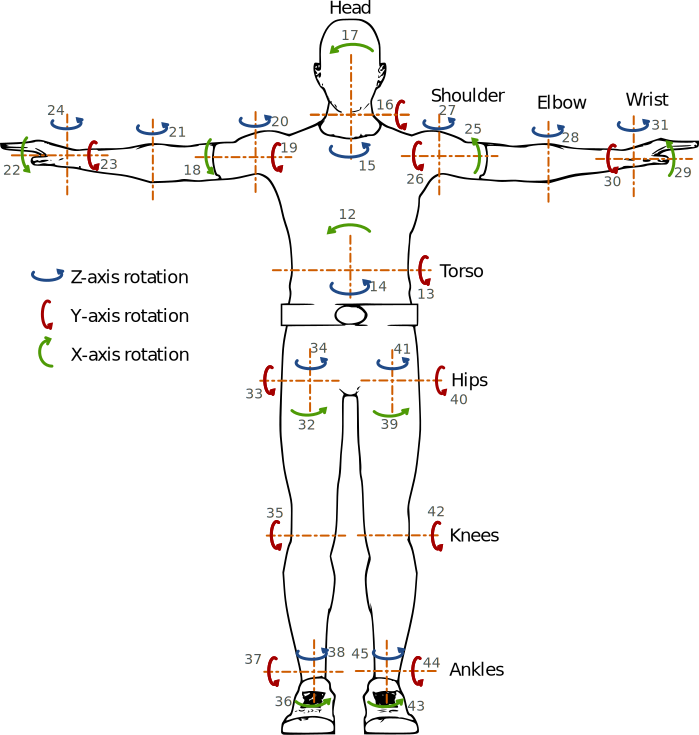
\includegraphics[width=0.45\linewidth]{human_joints}

        Joints values to cartesian positions: {\Medium forward kinematics}
        Cartesian positions to joints: {\Medium inverse kinematics}
    \end{center}
\end{frame}


\begin{frame}{Recognizing postures}
\end{frame}


{\paper{Images source: http://www.creativedistraction.com}
\begin{frame}{Gestures}
    \begin{center}
        \includegraphics[width=0.5\linewidth]{gesture-ideal}
        \includegraphics<2>[width=0.5\linewidth]{gesture-real}
    \end{center}
\end{frame}
}


{
\paper{Image source: Tdunning, CC-BY 3.0}
\begin{frame}{Hidden Markov Models}
    \begin{center}
        \includegraphics[width=0.5\linewidth]{hmm}
    \end{center}
    \only<1>{
    States: $s_1, s_2,...s_n$ {\scriptsize (eg, step of the gesture)}\\
    Observations: $o_1, o_2,...o_m$ {\scriptsize (eg, hand position)}\\
    State transition probabilities: $a_{ij}$\\
    Output probabilities: $b_{ij}$
}
\only<2>{
    Probabilities are learnt from examples: {\Medium supervised training}

    Very common for {\Medium temporal pattern recognition} (speech, handwriting,
    gestures...)
}

\end{frame}
}

\begin{frame}{Hidden Markov Models}
    We'll leave it here, but for the curious:\\
    \url{http://www.creativedistraction.com/demos/gesture-recognition-kinect-with-hidden-markov-models-hmms/}
\end{frame}

\begin{frame}{Attention}
\end{frame}


%%%%%%%%%%%%%%%%%%%%%%%%%%%%%%%%%%%%%%%%%%%%%%%%%%%%%%%%%%%%%%%%%%%%%%%
%%%%%%%%%%%%%%%%%%%%%%%%%%%%%%%%%%%%%%%%%%%%%%%%%%%%%%%%%%%%%%%%%%%%%%%
%%%%%%%%%%%%%%%%%%%%%%%%%%%%%%%%%%%%%%%%%%%%%%%%%%%%%%%%%%%%%%%%%%%%%%%

\section{One example: greetings recognizer}

\begin{frame}{Recognizing hand waving}
    \begin{itemize}
        \item Acquiring a depth image
        \item Extracting the skeleton
        \item Conversion to joint space
        \item Implementating an HMM
        \item Classifying incoming gestures
    \end{itemize}
\end{frame}


\end{document}






